\documentclass[11pt,a4paper]{article}
\usepackage[T1]{fontenc}
\usepackage{lmodern}
\usepackage[margin=25mm]{geometry}
\usepackage{booktabs,tabularx}
\usepackage{graphicx}
\usepackage{pdflscape}
\usepackage{tikz}
\usetikzlibrary{arrows.meta}
\usepackage[hidelinks]{hyperref}

\newcommand{\signuprevision}{e771a276aaf944f29ecfceb84d1276842f68055f}
\newcommand{\project}{https://github.com/bekadoux/cyberguard}
\newcommand{\code}[1]{\texttt{#1}}
\newcommand{\route}[1]{\nolinkurl{#1}}
\newcolumntype{Y}{>{\raggedright\arraybackslash}X}
\graphicspath{{docs/bpmn/}{../bpmn/}}

\hypersetup{
  pdftitle={CyberGuard: Project Technical Report},
  pdfsubject={Incident workflow, architecture, deployment and validation}
}

\title{\textbf{CyberGuard}\\[0.5em]\Large Project Technical Report}
\author{CyberGuard project team}
\date{}

\begin{document}
\maketitle

\begin{abstract}
CyberGuard is a self-hosted information system for reporting, investigating
and resolving cybersecurity incidents. It replaces fragmented reports and
follow-up messages with a case record, a staff assignee during investigation,
and separate reporter and staff views. A React client and Go API implement the
core workflow, with independent PostgreSQL instances for identity and incident
data. Optional local models help staff classify reports and prepare an
investigation brief. They cannot take response actions or decide outcomes.
This report distinguishes the integrated system on \code{main}, work on
other GitHub branches, and the limits of the available validation evidence.
\end{abstract}

{\small\tableofcontents}
\clearpage

\section{Purpose and scope}

An employee who reports a possible security incident needs to know whether
someone is handling it and whether more information is needed. The analyst
needs an assigned queue, a record of decisions and a private place for working
notes. CyberGuard brings those tasks together while limiting what each user
can read and change. It manages the case record; it does not detect attacks,
perform containment, or act as a general-purpose security agent.

Reports can be written in English or Slovak. The domain model uses one main
category from eight choices, including phishing, malware and an \code{other}
category. Staff set the confirmed severity on a four-level scale from low to
critical. New reports have no severity, and the domain's first-response
targets are guidance, not enforced service-level commitments.

\subsection{Repository scope}

The report covers the 15 GitHub branch tips reviewed for this edition.
The foundation, authentication, incident workflow, frontend, AI and
deployment histories are all accounted for in \code{main} at
\code{da6c4b8}: the other 13 already integrated feature-branch tips are
ancestors of that revision. The only non-integrated tip is
\route{feature/ai-signup-ui} at
\href{\project/commit/\signuprevision}{\code{e771a27}}. Its changes are
described separately below; the report does not assume they have been
merged, deployed or tested together with the current \code{main}.

\section{Incident workflow}

\subsection{Roles and permissions}

The API checks account role, incident assignment and reporter ownership
separately. An analyst can be the reporter of an incident; this does not make
the analyst its assignee.

\begin{center}
\begin{tabularx}{\linewidth}{@{}lY@{}}
\toprule
\textbf{Role} & \textbf{Responsibilities and visibility} \\
\midrule
Employee & Submit reports, read own cases, reply publicly, and confirm a
resolution or ask for review. No internal comments, staff audit or AI output. \\
\addlinespace
Analyst & Read the company queue, claim unassigned reports, write internal
notes, and read assessments. Update confirmed fields, make staff transitions
and review AI output on cases assigned to them, subject to workflow rules. \\
\addlinespace
Administrator & Handle incidents, assign or reassign an eligible analyst,
reopen closed or false-positive cases, archive with a reason, and administer
accounts. May read the account audit. \\
\bottomrule
\end{tabularx}
\end{center}

\subsection{Lifecycle and communication}

\begin{enumerate}
  \item \textbf{Submission and triage.} Any active role can submit a report.
    The initial state is \code{submitted}. A successful staff claim or
    first admin assignment moves it to \code{triage}. Competing claims cannot
    both succeed.
  \item \textbf{Investigation.} Staff set category and severity before moving
    the case to \code{investigating}. A false positive can be recorded from
    triage with a reason. During an investigation, a staff member can move
    the case to \code{awaiting\_reporter} after posting a public question
    in the current investigation cycle, while it remains unanswered.
    A public reply from the reporter returns it to
    \code{investigating}; internal notes do not count.
  \item \textbf{Resolution and closure.} Staff record the outcome and move the
    case to \code{resolved}. The reporter can confirm it to close the case,
    or reopen the investigation by requesting review or posting a public
    reply. Unanswered resolutions become eligible for closure after seven
    days; Go checks at startup and hourly. An admin can reopen a closed or
    false-positive incident with a reason. Archiving is separate from status.
\end{enumerate}

Public comments support the discussion with the reporter; internal notes and
the staff action history are separate. Go records workflow actions and sends
in-app notifications for events such as assignment, status changes and
public replies. Account changes have their own audit history.

\subsection{Business process model}

The BPMN diagrams in Appendix~\ref{app:bpmn} show the main process and its
investigation-and-response subprocess. The company pool has lanes for the
employee, system, analyst and administrator or security manager. A second
pool represents an external security provider.
The diagrams show the question-and-reply loop, the closure timer and reopening.
They also describe activities outside the application, such as external
escalation, management communication, response measures and preparation for
possible regulatory notification. CyberGuard records or supports those
activities; it does not automate them. The domain specification identifies
application paths the diagrams simplify, including archiving and admin
assignment.

\section{System architecture}

\begin{figure}[htbp]
\centering
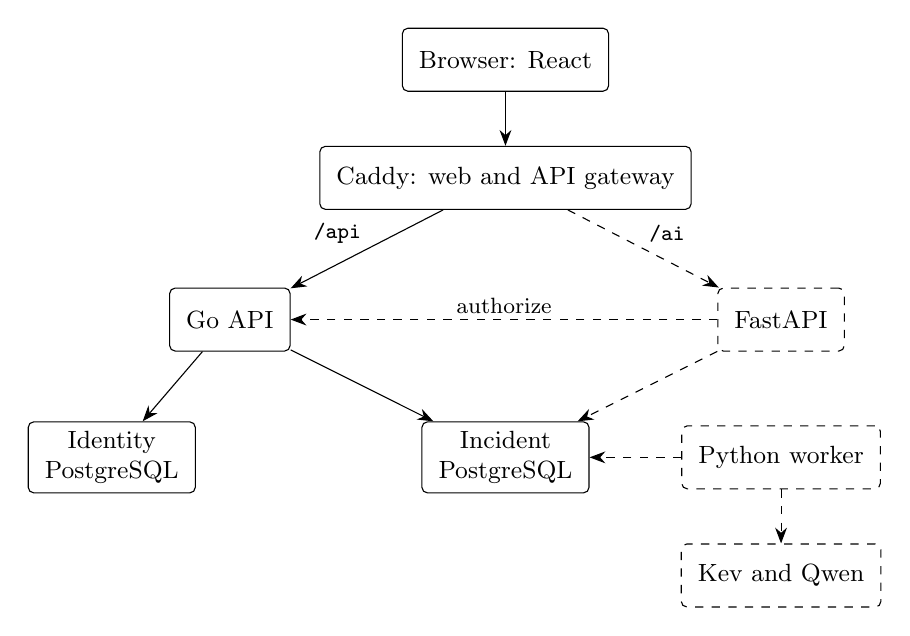
\begin{tikzpicture}[
  component/.style={draw,rounded corners=2pt,align=center,
    minimum height=8mm,inner xsep=6pt,font=\small},
  optional/.style={component,dashed},
  flow/.style={-{Stealth[length=2mm]}},
  labeltext/.style={font=\footnotesize,fill=white,inner sep=2pt}
]
  \node[component] (browser) at (0,3.3) {Browser: React};
  \node[component] (gateway) at (0,1.8) {Caddy: web and API gateway};
  \node[component] (go) at (-3.5,0) {Go API};
  \node[optional] (ai) at (3.5,0) {FastAPI};
  \node[component] (identity) at (-5,-1.75) {Identity\\PostgreSQL};
  \node[component] (incident) at (0,-1.75) {Incident\\PostgreSQL};
  \node[optional] (worker) at (3.5,-1.75) {Python worker};
  \node[optional] (models) at (3.5,-3.25) {Kev and Qwen};
  \draw[flow] (browser) -- (gateway);
  \draw[flow] (gateway) -- node[labeltext,above left] {\code{/api}} (go);
  \draw[flow,dashed] (gateway) --
    node[labeltext,above right] {\code{/ai}} (ai);
  \draw[flow] (go) -- (identity);
  \draw[flow] (go) -- (incident);
  \draw[flow,dashed] (ai) -- node[labeltext,above] {authorize} (go);
  \draw[flow,dashed] (ai) -- (incident);
  \draw[flow,dashed] (worker) -- (incident);
  \draw[flow,dashed] (worker) -- (models);
\end{tikzpicture}
\caption{Core components and optional AI paths (dashed). The worker also reads
the job's saved report snapshot from private Go routes.}
\label{fig:architecture}
\end{figure}

Figure~\ref{fig:architecture} shows the logical service boundaries, which
are the same on one development host or across deployed VMs.

\begin{description}
  \item[React and Caddy.] Vite builds the React/TypeScript single-page app
    into static assets; Node is not a runtime service. Caddy serves the UI
    and routes credentialed requests from one browser origin. The UI provides
    login, incident submission, a filtered queue, detail and workflow forms,
    comments, notifications, administration and a staff AI assessment panel.
    Access checks in the UI improve navigation but do not replace server checks.
  \item[Go.] The Go service owns identity, sessions and incident mutations.
    Chi routes browser requests to handlers; pgx pools and sqlc-generated
    query bindings provide access to the two PostgreSQL instances.
  \item[Python.] FastAPI serves stored assessments after checking authorization
    with Go. A separate worker claims and processes queued assessments,
    independent of the submitting browser. Model servers are private.
\end{description}

\section{Data, APIs and security}

\subsection{Storage and transaction boundaries}

\begin{center}
\begin{tabularx}{\linewidth}{@{}lYY@{}}
\toprule
\textbf{Instance} & \textbf{Stored data} & \textbf{Runtime access} \\
\midrule
Identity & Users and password hashes, sessions, application ownership and
account audit & Go only \\
\addlinespace
Incidents & Case records, resolution timers, comments, actions,
notifications, immutable snapshots, AI jobs and results & Go and a
restricted Python role for approved job/result operations \\
\bottomrule
\end{tabularx}
\end{center}

The databases run on separate PostgreSQL instances. Incident records refer
to users by UUID without cross-instance foreign keys or transactions. For
example, an admin's assignment checks the target's eligibility in identity
before the incident transaction; those operations are not one atomic change
across both systems.

A report insert atomically creates its submission event, immutable input
snapshot and one initial assessment job, even when AI is disabled.
Later edits do not rewrite that input. Human AI feedback is recorded
separately from model output; accepting or correcting the category commits
the category change and review together. Goose tracks the separate schema
chains, at identity \code{00005} and incidents \code{00010} for this
baseline. Bootstrap, migration and runtime roles have separate privileges.

\subsection{API and privacy boundaries}

The following paths are shown as the browser sees them through Caddy. The
gateway removes \route{/api} or \route{/ai} before forwarding to the service.

\begin{center}
\begin{tabularx}{\linewidth}{@{}lY@{}}
\toprule
\textbf{Surface} & \textbf{Contract} \\
\midrule
\route{/api/auth/...} & Signup, login, current session and logout. \\
\addlinespace
\route{/api/incidents} & Submission and scoped list. The list filters by
status and category and uses cursor pagination. Staff rows carry
\route{ai_assessment_status} for the initial job, including on their own
reports. A missing initial job is represented as \code{null}; employee
rows omit the field entirely. \\
\addlinespace
\route{/api/incidents/{id}/...} & Detail, workflow actions, comments and
separate staff history. The reporter-only \route{/timeline} returns paginated
status and UTC timestamp pairs, newest first. \\
\addlinespace
\route{/api/notifications} & In-app inbox and per-notification read state
for the current user. \\
\addlinespace
\route{/api/admin/...} & Account administration, ownership transfer,
account audit and feature-gated demo incident creation. \\
\addlinespace
\route{/ai/incidents/{id}/assessment} & Initial job status and stored
assessment for authorized staff. FastAPI asks Go to check both the current
account and incident visibility before reading the result. \\
\bottomrule
\end{tabularx}
\end{center}

The timeline never exposes actors, reasons, audit IDs, comments, AI output or
reassignments. It shows the submission and reliably recorded status changes;
it does not reconstruct old transitions from assignment records. Non-owners
and archived, missing or invalid incident IDs get the same \code{404} for
this endpoint; absent or invalid sessions get \code{401}. The endpoint
applies the ownership check again on every page, including for staff.
The incident-list status does not expose a job ID or model output and does
not require a live Python service. These two Go contracts are merged. Their
dedicated UI surfaces are follow-ups: \href{\project/issues/16}{reporter
status history} and the \href{\project/issues/17}{staff queue column}.

\subsection{Session and account protection}

Passwords are hashed with Argon2id. The browser holds an opaque, host-only
\code{HttpOnly} cookie (also \code{Secure} in deployment); the session lives
in the identity database. The defaults are an eight-hour absolute limit and
a 30-minute idle limit. The server checks current role, blocked state and
the account's authentication version on each protected request. Role,
password and block-state changes invalidate existing sessions. Exact trusted
origins and CSRF checks protect browser writes.

Session refresh updates only a still-present, unexpired record. It cannot
insert a previously loaded token after concurrent logout or revocation.
Only successful explicit login or logout changes the browser cookie.
Incident requests refresh before acting and do not save a session after a
business write, so a late session failure cannot turn an already committed
write into a session error.

Signup is off by default. If enabled, it creates only an active employee
account and does not sign it in. At the baseline it is available through the
API, not a sign-up page in the main branch. A deployment operator initializes
one active administrator as application owner. Other admins cannot block,
demote or reset the owner. Transfer requires the owner's current password
and another active administrator; the former owner remains an ordinary
administrator.

\section{AI-assisted assessment}

\subsection{Job execution}

The worker verifies its own service credential with private Go, claims a job
with a renewable lease and receives the saved report snapshot through Go.
Python has no identity database access and cannot read report descriptions
directly from incident tables. Token and lease checks prevent stale claims
from committing results; PostgreSQL stores the result and marks the job
complete together. Recovery from an expired lease is bounded, and a terminal
failure is not retried automatically. Snapshot-less pending legacy jobs
require an explicit operator decision before the worker can become ready.

Job states (\code{queued}, \code{running}, \code{completed}, \code{failed})
are independent of the incident lifecycle. \code{completed} means processing
finished, not that the model made a category recommendation or that a
human reviewed it. A queued job can remain queued while AI is offline.
Core submission and investigation do not depend on AI availability.

\subsection{Model output and human decision}

\begin{description}
  \item[Kev-0.8B] on \code{main} produces category probabilities, a separate
    0--3 potential impact score and four signals: link clicked, credentials entered,
    files encrypted and unauthorized access reported. No category is
    suggested when \code{other} wins or the top score falls below the
    provisional 0.60 threshold. These scores are not calibrated risk
    estimates or confirmed severity. The eight-question domain rubric
    covers a different set of indicators. The unmerged branch aligns the
    prompts and staff display with that rubric.
  \item[Qwen2.5-1.5B-Instruct] runs through llama.cpp on CPU and produces a
    draft brief with a summary, reported facts, unknowns and follow-up
    questions. Report text is untrusted input. The model cannot call tools.
    Up to four suggested response steps come from checked-in playbooks,
    not model-generated actions.
\end{description}

Staff refresh assessments manually. For a real assessment on an eligible
incident, the assigned analyst or an admin can record one accept, correct
or reject decision. Acceptance or correction updates the confirmed
category; rejection leaves it unchanged. Severity remains a separate
human action. Fixture results are labelled and cannot be reviewed as real
assessments.

\section{Changes on the unmerged branch}

\href{\project/pull/14}{PR~14} proposes an update across React, Caddy and the
Python assessment contract. The changes below are implemented on its
branch, not in the integrated build:

\begin{itemize}
  \item A \route{/signup} page and Caddy route use the existing Go signup API.
    The form validates input and handles disabled registration, duplicate
    names, rate limits and network errors. Registration still creates only
    an employee account and requires a separate sign-in; the feature flag
    remains off by default.
  \item Kev's prompts use the domain's eight explicitly reported indicators
    and clarify category boundaries. The changed assessment contract and UI
    can still read legacy scores from stored rows. A low indicator score is
    not evidence an event did not occur. The 0.60 category threshold remains
    provisional, and no calibrated indicator decision threshold is provided.
  \item The staff panel separates recommendations from abstentions, ranks
    category scores, and separates the AI brief from approved playbook steps.
    The review UI keeps Accept, Correct and Reject distinct; if the model
    abstains, staff choose a category rather than accept one.
\end{itemize}

This branch does not implement the reporter timeline or the staff queue
status column in React. Its registration and assessment changes must be
integrated with the current Go and Caddy contracts and verified together
before release.

\section{Deployment and operations}

\begin{description}
  \item[Local Docker.] The base development stack uses Caddy, Go and both
    PostgreSQL instances, with an HTTP entry point at
    \route{http://127.0.0.1:8088/login}. The optional local AI stack adds FastAPI,
    the worker and private CPU inference. The runbook separates secret
    generation, builds, database provisioning, migrations and demo seeding.
    Local HTTP/demo configuration is not intended for internet exposure.
  \item[Azure application VM.] Public Caddy serves HTTPS, static assets and
    public API routes. Go is not published directly. Both PostgreSQL instances
    use verified TLS and persistent data volumes. Public TLS certificate
    state is persistent. The identity database is not reachable from the AI VM.
  \item[Optional Azure AI VM.] Private Caddy exposes FastAPI to the application
    VM over verified TLS. The approved AI VM reaches only the permitted
    private Go reads and the restricted incident SQL endpoint across VMs.
    The model services and worker run on the AI VM; it does not host a
    database or a public frontend.
\end{description}

Operators provide Azure resources, network rules, private DNS and TLS
materials. Compose mounts scoped file secrets; database administrator and
migration credentials do not go to the AI VM. Model preparation is explicit:
normal startup does not download weights, run migrations or seed accounts.
Fresh deployments initialize the application owner; upgrades use the
maintenance and migration procedure rather than regenerating secrets or
removing volumes. The workstation SSH tooling helps set up fresh VMs but
does not provision cloud resources or perform in-place upgrades.

The local and VM runbooks are the operational sources of truth. In
particular, incidents migration \code{00010} must be applied before
starting the baseline Go API with its staff list projection.

\section{Validation and limitations}

\subsection{What the available checks establish}

\begin{center}
\begin{tabularx}{\linewidth}{@{}lY@{}}
\toprule
\textbf{Check} & \textbf{Scope and evidence} \\
\midrule
Go HTTP and SQL &
The \href{\project/pull/15}{incident-view PR} records passing focused
Go/race checks and integration tests against two disposable PostgreSQL
instances. Coverage includes role-specific list fields and filters,
reporter-only timeline access, and pagination with tied timestamps. The
\href{\project/commit/868c79f}{follow-up tests} cover claim, public reply
and auto-closure in the reporter view. \\
\addlinespace
Contracts and frontend &
The same PR records OpenAPI and sqlc checks for the changed Go contracts.
Frontend unit/component and browser suites are documented separately;
default browser tests use synthetic API responses. Packaged-browser
checks can also exercise real same-origin service flows in Docker. \\
\addlinespace
AI and deployment fixtures &
Python unit tests can use mocked HTTP dependencies. Disposable smoke
fixtures exercise real service and database wiring, including TLS in
deployment fixtures, with synthetic model responses. This tests
integration, not real inference quality, capacity or Azure behavior. \\
\bottomrule
\end{tabularx}
\end{center}

The repository defines check entry points in the \code{Makefile}.
The presence of a target does not mean
that it ran successfully on this baseline.

\subsection{Open validation and follow-ups}

\begin{itemize}
  \item The reference dataset contains 80 labelled synthetic descriptions
    (61 English and 19 Slovak). It is not a measured model result. Model
    assessment still needs reviewed category and indicator metrics,
    uncertainty/calibration checks and evidence that generated briefs
    distinguish reported facts from unsupported claims.
  \item A target-host rehearsal with real Kev and Qwen should verify the
    end-to-end workflow, AI outage behavior and resource use. Azure
    network rules, public certificate issuance and renewal, reboot
    persistence, restore and credential rotation need separate acceptance.
  \item Staged worker recovery behavior, including competing claims and
    lease expiry in the deployed configuration, still needs explicit
    validation. Current process-local login limits and the in-process
    closure scheduler are not a multi-replica operating plan.
  \item The two incident-view UI follow-ups remain open. The sign-up and AI
    UI branch adds frontend and model-contract checks, but does not demonstrate
    integrated acceptance on the current \code{main}, real model quality, or
    readiness for public registration.
\end{itemize}

\section{Conclusion}

CyberGuard provides a case workflow that works without AI. Its main design
choices are explicit ownership, separate views for reporters and staff,
server-side authorization, and independent persistence for identity and
incidents. Optional AI reads an immutable submission and provides advice
without taking over the case. The implemented interfaces and focused
integration checks support that design; they do not establish production
readiness or model quality.

\clearpage
\appendix
\begin{landscape}
\section{BPMN diagrams}
\label{app:bpmn}
The original diagrams use Slovak labels. The first follows a report from
submission through triage, investigation, resolution and closure. The second
expands the investigation and response subprocess, including conditional
containment activities and coordination with an external security provider.
Zoom in to read individual activities and gateways.

\begin{figure}[htbp]
\centering
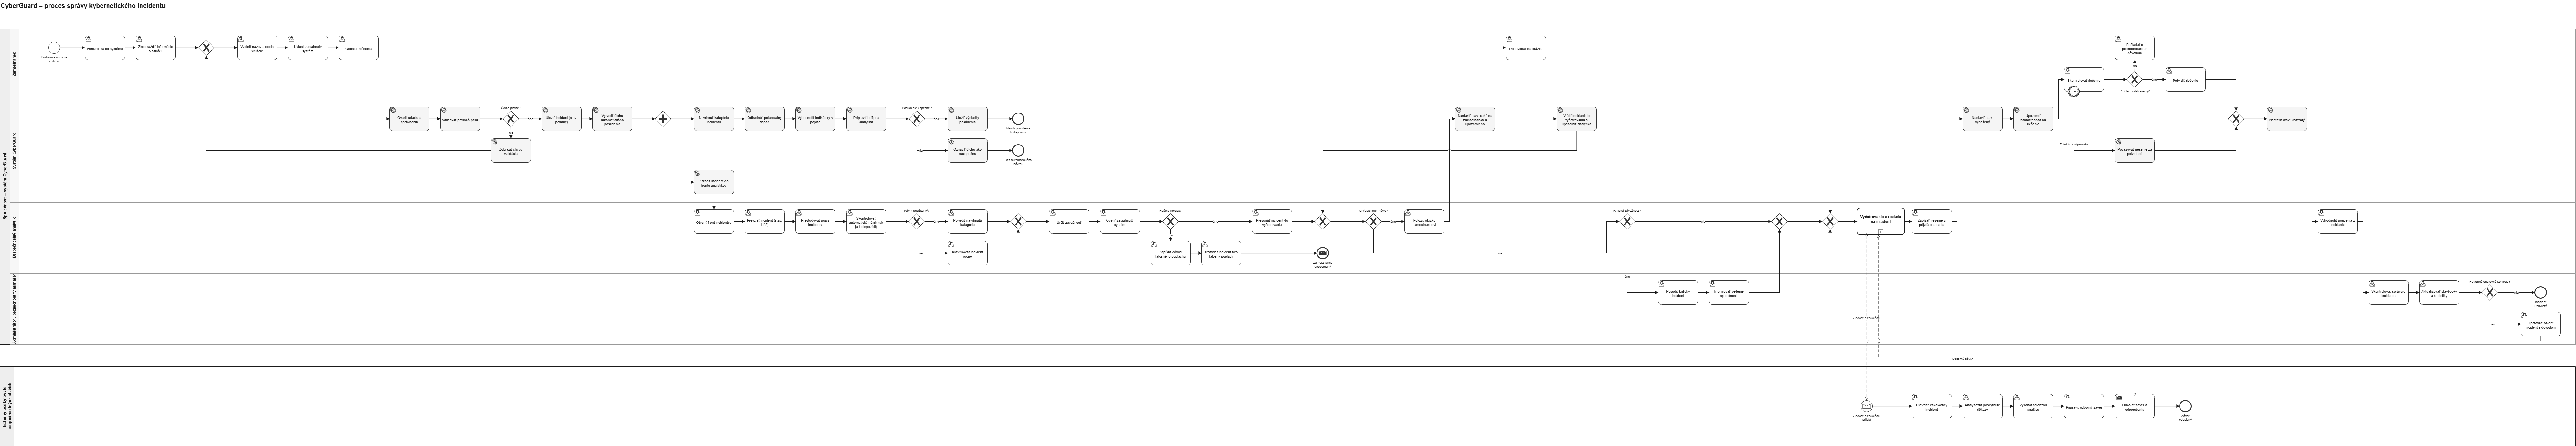
\includegraphics[width=\linewidth]{CyberGuard_BPMN Hlavný proces.drawio.png}
\caption{Main CyberGuard incident-handling process.}
\label{fig:bpmn-main}
\end{figure}

\begin{figure}[htbp]
\centering
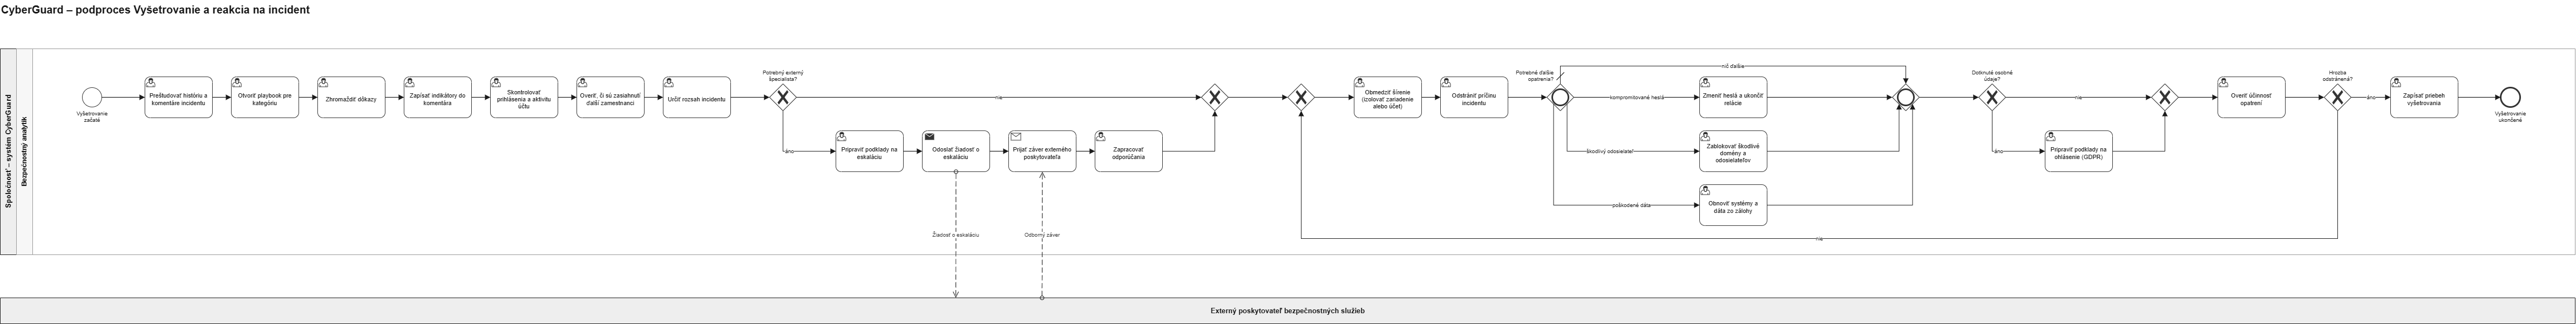
\includegraphics[width=\linewidth]{CyberGuard_BPMN Podproces – vyšetrovanie a reakcia.drawio.png}
\caption{Investigation and response subprocess.}
\label{fig:bpmn-investigation}
\end{figure}
\end{landscape}

\end{document}
